% The Unique Intersection of Probability and Many-Valued Logic
% Publication-quality paper
%
% References to Lean formalization: lean/Cred/Basic.lean

\documentclass[11pt,a4paper]{article}

\usepackage{amsmath,amssymb,amsthm}
\usepackage{mathtools}
\usepackage{enumitem}
\usepackage{booktabs}
\usepackage{caption}
\usepackage{hyperref}
\hypersetup{
    colorlinks=true,
    linkcolor=blue,
    citecolor=blue,
    urlcolor=blue,
    pdfauthor={Anonymous},
    pdftitle={The Unique Intersection of Probability and Many-Valued Logic}
}
\usepackage{cleveref}
\usepackage[margin=1in]{geometry}
\usepackage{tikz}
\usetikzlibrary{arrows.meta,positioning,shapes}
\usepackage{graphicx}

% Theorem environments
\newtheorem{theorem}{Theorem}[section]
\newtheorem{lemma}[theorem]{Lemma}
\newtheorem{proposition}[theorem]{Proposition}
\newtheorem{corollary}[theorem]{Corollary}
\newtheorem{definition}[theorem]{Definition}
\newtheorem{example}[theorem]{Example}
\newtheorem{remark}[theorem]{Remark}

% Custom commands
\newcommand{\cred}{\mathsf{cred}}
% \newcommand{\Cred}{\mathsf{Cred}} % removed: no branding
\newcommand{\negc}{\mathord{\sim}}
\newcommand{\conjc}{\otimes}
\newcommand{\disjc}{\sqcup}
\newcommand{\condc}[2]{({#1} \mid {#2})}
\newcommand{\Real}{\mathbb{R}}
\newcommand{\Nat}{\mathbb{N}}

\title{\textbf{The Unique Intersection of Probability and Many-Valued Logic}}

\author{Anonymous for blind review}
\date{February 2026}

\begin{document}

\maketitle

\begin{abstract}
We prove two results about truth-functional conjunctions on $[0,1]$.
First, $\min(a,b)$ is the unique conjunction satisfying Bayes consistency,
non-trivial conditioning, and idempotence---this forces the Kleene conjunction
used in K$_3$, LP, and RM3.
Second, the conditional's limit at evidence zero is path-dependent (like the
Borel--Kolmogorov paradox), so ex falso requires an added convention.
The framework uses credences in $[0,1]$, complement $1-c$, and the chain rule
$\cred(A \mid B) \cdot \cred(B) = \cred(A \land B)$.
A collapse homomorphism to the Kleene lattice exists; none exists for
G\"odel or \L ukasiewicz.
Proofs are machine-checked in Lean~4.
\end{abstract}

%=============================================================================
\section{Introduction}
\label{sec:intro}
%=============================================================================

A \emph{credence} is a real number in $[0,1]$ representing degree of belief~\cite{ramsey1931,definetti1937,jaynes2003}.
Probability theory builds on credences by adding a sigma-algebra, a measure, and sigma-additivity.
Conditional probability is derived via division: $P(A \mid B) = P(A \land B)/P(B)$ when $P(B) > 0$; when $P(B) = 0$, the ratio is undefined.
R\'enyi~\cite{renyi1955} and Popper~\cite{popper1959} proposed an alternative: treat conditioning as \emph{primitive}, governed by the chain rule $P(A \mid B) \cdot P(B) = P(A \land B)$ without invoking division.

The credence algebra takes this further.
Drop the measure entirely; keep only values in $[0,1]$, the complement $\negc c = 1 - c$, and the chain rule $\cred(A \mid B) \cdot \cred(B) = \cred(A \land B)$ as the sole structural axiom for conditioning.
This is strictly weaker than probability: every probability space satisfies these axioms, but the algebra requires neither a sigma-algebra nor additivity.
The conjunction is the product t-norm, the disjunction its De Morgan dual (the probabilistic sum), and together with complement they form the \emph{product De Morgan triplet}~\cite{klement2000,hajek1998}.

The key design choice concerns conditioning at evidence zero.
In t-norm fuzzy logic, each conjunction determines a unique implication via \emph{residuation}: $a \to b = \sup\{c : a \otimes c \leq b\}$.
Since $0 \otimes c = 0 \leq b$ for all $c$ and $b$, every residuated implication forces $0 \to b = 1$---\emph{ex falso quodlibet} is built in~\cite{hajek1998}.
The chain rule avoids this: $c \cdot 0 = 0$ is satisfied by \emph{any} value of $c$, so conditioning on impossible evidence is unconstrained.
A concrete example: ``if the moon is made of cheese, then my birthday is tomorrow'' is vacuously true under material implication, but the chain rule imposes no constraint when the antecedent has credence zero.
This echoes de Finetti's three-valued conditional~\cite{definetti1936}, where conditioning on a false antecedent yields \emph{void} rather than vacuous truth.

\textbf{Main results.}
\begin{enumerate}[label=(\arabic*)]
\item \textbf{Uniqueness of min} (Theorem~\ref{thm:uniqueness-main}):
  Among truth-functional conjunctions on $[0,1]$, only $\min(a,b)$ satisfies Bayes consistency, non-trivial conditioning, and idempotence.
  This forces the Kleene conjunction used in K$_3$, LP, and RM3.
\item \textbf{Path dependence at zero} (Theorem~\ref{thm:path-dependence}):
  The conditional's limit as evidence $\to 0$ depends on the ratio of joint to evidence---the same structure as the Borel--Kolmogorov paradox.
  Ex falso requires an added convention.
\item \textbf{Collapse to Kleene} (Theorem~\ref{thm:collapse}):
  A surjective homomorphism from the credence algebra to the Kleene lattice exists for $\{\negc, \conjc, \disjc\}$; no analogous collapse exists for G\"odel, \L ukasiewicz, or classical logic.
\item \textbf{Bayes consistency} as selection criterion: the product residuated implication passes; RM3 and G\"odel fail (Section~\ref{sec:relationships}).
\item \textbf{Lean formalization}: Proofs are machine-checked in Lean~4 (Appendix~\ref{app:lean}).
\end{enumerate}

\textbf{Scope.}
The credence algebra is a constraint algebra on $[0,1]$: it specifies how credence values must relate through the product, complement, and chain rule.
It has no interpretation (no map from propositions to credences), no consequence relation, and no update rule---like Boolean algebra before propositional logic adds valuations, or $[0,1]$ arithmetic before probability adds a measure space.
Part~2~\cite{part2} extends the algebra to valuations, consequence relations, and update rules.

\textbf{Outline.}
Section~\ref{sec:algebra} defines the algebra.
Section~\ref{sec:uniqueness} proves uniqueness of min (Main Result~1).
Section~\ref{sec:conditioning} develops primitive conditioning and path dependence (Main Result~2).
Section~\ref{sec:fixed-points} treats fixed points.
Section~\ref{sec:collapse} establishes the collapse to the Kleene lattice.
Section~\ref{sec:relationships} relates the algebra to existing frameworks.
Section~\ref{sec:conclusion} concludes.
Appendix~\ref{app:prelim} provides formal preliminaries.
Appendix~\ref{app:extended} contains extended comparisons.
Appendix~\ref{app:lean} describes the Lean formalization.

%=============================================================================
\section{The Credence Algebra}
\label{sec:algebra}
%=============================================================================

\subsection{Primitive Operations}

\begin{definition}[Credence]
\label{def:credence}
A \emph{credence} is a real number $c \in [0, 1]$.
The set of credences is $[0, 1] \subset \Real$.
\end{definition}

\begin{definition}[Negation]
\label{def:neg}
The \emph{negation} of $c$ is $\negc c = 1 - c$.
\end{definition}

Negation is the standard complement: if we assign credence $0.7$ to proposition $A$,
we assign credence $0.3$ to its negation.

\begin{definition}[Product]
\label{def:conj}
The \emph{product} of $c_1$ and $c_2$ is $c_1 \conjc c_2 = c_1 \cdot c_2$.
\end{definition}

The product is multiplication on $[0,1]$---the same operation that appears in the
chain rule (Section~\ref{sec:conditioning}).
It is the product t-norm of fuzzy logic~\cite{klement2000}.

\textbf{Important distinction.}
The product $c_1 \conjc c_2$ is an \emph{algebraic operation} on credence values.
It is \emph{not} a claim about the actual joint credence $\cred(A \land B)$ of
two propositions $A$ and $B$.
The joint credence of two propositions depends on their dependence structure:
\begin{itemize}[nosep]
\item Under independence: $\cred(A \land B) = \cred(A) \cdot \cred(B)$.
  This gives \emph{trivial conditioning}: $\cred(A \mid B) = \cred(A)$---evidence
  has no effect.
\item Under maximum positive dependence: $\cred(A \land B) = \min(\cred(A), \cred(B))$
  (Fr\'echet upper bound).
  This gives \emph{non-trivial, Bayes-consistent conditioning}---this is what
  three-valued logic uses, and is the unique choice satisfying both requirements.
\item Under maximum negative dependence: $\cred(A \land B) = \max(\cred(A) + \cred(B) - 1, 0)$
  (Fr\'echet lower bound---the \L ukasiewicz t-norm).
\end{itemize}
The credence algebra does not commit to any particular dependence structure.
The joint credence $\cred(A \land B)$ is an \emph{external parameter} that can
take any value in the Fr\'echet-Hoeffding interval
$[\max(\cred(A) + \cred(B) - 1, 0),\; \min(\cred(A), \cred(B))]$.
The chain rule relates this joint to conditioning:
$\cred(A \mid B) \conjc \cred(B) = \cred(A \land B)$.
Different dependence assumptions yield different conditioning behaviors;
the algebra supports all of them.

\begin{definition}[Disjunction]
\label{def:disj}
The \emph{disjunction} of $c_1$ and $c_2$ is defined via De Morgan duality:
\[
c_1 \disjc c_2 = \negc(\negc c_1 \conjc \negc c_2) = c_1 + c_2 - c_1 \cdot c_2
\]
\end{definition}

The symbol $\disjc$ denotes the De Morgan dual of the product, not a
lattice join (which would be idempotent).
The triple $(\conjc, \disjc, \negc)$ is the \emph{product De Morgan triplet}:
conjunction is the product t-norm, disjunction its dual t-conorm (the
``probabilistic sum''), and negation the standard
complement~\cite{klement2000,hajek1998}.
These operations are truth-functional---determined entirely by the operand
values---which is what makes the collapse homomorphism to the Kleene lattice
possible (Section~\ref{sec:collapse}).

\begin{remark}[Credence vs.\ Probability]
\label{rem:not-probability}
The credence algebra's core consists of three ingredients: values in $[0,1]$, the complement
$\negc c = 1 - c$, and the chain rule for conditioning.
Probability adds a sigma-algebra, a measure, and sigma-additivity; every
probability space therefore satisfies the credence algebra's axioms, making probability a
special case.
In probability, the joint $P(A \land B)$ is determined by the measure---not
by the product of marginals (unless events are independent).
The credence algebra makes no such determination: $c_1 \conjc c_2$ is multiplication on
$[0,1]$, not a claim about the actual joint of arbitrary propositions.
The actual joint is an external input to conditioning.
The credence algebra's disjunction $c_1 \disjc c_2 = c_1 + c_2 - c_1 c_2$ is the De Morgan
dual of the product; probability's inclusion-exclusion
$P(A \lor B) = P(A) + P(B) - P(A \land B)$ uses the actual joint instead.
\end{remark}

\subsection{Algebraic Properties}

% Lean: neg_neg, neg_zero, neg_one, conj_comm, conj_assoc, conj_one, conj_zero,
%       disj_comm, disj_assoc, disj_zero, disj_one, de_morgan_conj, de_morgan_disj
\begin{theorem}[Algebraic Properties]
\label{thm:algebraic}
The following hold for all $c, c_1, c_2, c_3 \in [0,1]$:
\begin{enumerate}[label=(\alph*)]
\item $\negc\negc c = c$ \hfill (involution)
\item $\negc 0 = 1$, $\negc 1 = 0$ \hfill (boundary)
\item $c_1 \conjc c_2 = c_2 \conjc c_1$, $(c_1 \conjc c_2) \conjc c_3 = c_1 \conjc (c_2 \conjc c_3)$ \hfill (comm., assoc.)
\item $c \conjc 1 = c$, $c \conjc 0 = 0$ \hfill (identity, annihilator)
\item $c_1 \disjc c_2 = c_2 \disjc c_1$, $(c_1 \disjc c_2) \disjc c_3 = c_1 \disjc (c_2 \disjc c_3)$ \hfill (comm., assoc.)
\item $c \disjc 0 = c$, $c \disjc 1 = 1$ \hfill (identity, annihilator)
\item $\negc(c_1 \conjc c_2) = \negc c_1 \disjc \negc c_2$, $\negc(c_1 \disjc c_2) = \negc c_1 \conjc \negc c_2$ \hfill (De Morgan)
\end{enumerate}
\end{theorem}
\begin{proof}
Each property follows directly from the definitions.
Lean verification: \texttt{neg\_neg}, \texttt{neg\_zero}, \texttt{neg\_one},
\texttt{conj\_comm}, \texttt{conj\_assoc}, \texttt{conj\_one}, \texttt{conj\_zero},
\texttt{disj\_comm}, \texttt{disj\_assoc}, \texttt{disj\_zero}, \texttt{disj\_one},
\texttt{de\_morgan\_conj}, \texttt{de\_morgan\_disj}.
\end{proof}

The structure $([0,1], \conjc, \disjc, \negc, 0, 1)$ consists of two dual
commutative monoids ($([0,1], \conjc, 1)$ and $([0,1], \disjc, 0)$) connected
by an involution $\negc$ that reverses the natural order on $[0,1]$
($c_1 \leq c_2$ iff $\negc c_2 \leq \negc c_1$) and satisfies
De Morgan's laws.
It is not a De Morgan algebra in the lattice-theoretic sense: a De Morgan
algebra requires a distributive lattice, whose meet and join are
idempotent, but $\conjc$ is not idempotent (Theorem~\ref{thm:idempotence})
and distributivity fails (Theorem~\ref{thm:nondistrib}).
Throughout this paper, ``the credence algebra'' refers to this concrete algebra on
$[0,1]$---a carrier, three operations, and the chain rule.
It is not a logic: there is no consequence relation, no designated truth
values, and no notion of valid inference.
Those require additional structure (Section~\ref{sec:conclusion}).

\subsection{Non-Idempotence and Non-Distributivity}

Unlike the two-element Boolean algebra $\{0,1\}$, the credence algebra is neither
idempotent nor distributive.

% Lean: conj_idempotent_iff
\begin{theorem}[Idempotence Characterization]
\label{thm:idempotence}
$c \conjc c = c$ if and only if $c \in \{0, 1\}$.
\end{theorem}
\begin{proof}
$c^2 = c$ iff $c(c-1) = 0$ iff $c \in \{0,1\}$.
In particular, $\tfrac{1}{2} \conjc \tfrac{1}{2} = \tfrac{1}{4} \neq \tfrac{1}{2}$.
Lean: \texttt{conj\_idempotent\_iff}.
\end{proof}

The product $c \conjc c = c^2$ is the credence of two \emph{independent} copies
of a proposition with credence $c$---not the credence of ``$A \land A$'' (which
equals $\cred(A)$).

% Lean: conj_disj_not_distrib
\begin{theorem}[Non-Distributivity]
\label{thm:nondistrib}
The product does not distribute over disjunction.
\end{theorem}
\begin{proof}
Counterexample at $c_1 = c_2 = c_3 = \tfrac{1}{2}$:
\begin{align*}
\text{LHS} &= \tfrac{1}{2} \conjc (\tfrac{1}{2} \disjc \tfrac{1}{2})
= \tfrac{1}{2} \cdot (\tfrac{1}{2} + \tfrac{1}{2} - \tfrac{1}{4})
= \tfrac{1}{2} \cdot \tfrac{3}{4} = \tfrac{3}{8} \\
\text{RHS} &= (\tfrac{1}{2} \conjc \tfrac{1}{2}) \disjc (\tfrac{1}{2} \conjc \tfrac{1}{2})
= \tfrac{1}{4} \disjc \tfrac{1}{4}
= \tfrac{1}{4} + \tfrac{1}{4} - \tfrac{1}{16} = \tfrac{7}{16}
\end{align*}
Lean: \texttt{conj\_disj\_not\_distrib}.
\end{proof}

Absorption likewise fails: $c \conjc (c \disjc d) \neq c$ in general
(e.g., $\tfrac{1}{2} \conjc (\tfrac{1}{2} \disjc \tfrac{1}{2}) =
\tfrac{1}{2} \cdot \tfrac{3}{4} = \tfrac{3}{8} \neq \tfrac{1}{2}$).
These failures of distributivity and absorption distinguish the credence algebra from
Boolean algebra and from De Morgan lattices.

%=============================================================================
\section{The Uniqueness Theorem}
\label{sec:uniqueness}
%=============================================================================

This section establishes the first main result: the minimum conjunction
$\min(a,b)$ is the \emph{unique} truth-functional joint compatible with
probabilistic marginalization that satisfies basic requirements for reasoning.
This is not a design choice---it is mathematically forced.

\subsection{The Problem: Fixing the Joint}

The product $c_1 \conjc c_2 = c_1 \cdot c_2$ is an algebraic operation on
credence values.
But what is the \emph{actual} joint credence $\cred(A \land B)$ of two
propositions?
In probability, the joint depends on the dependence structure between events.
In logic, we want a truth-functional answer: $\cred(A \land B)$ should depend
only on $\cred(A)$ and $\cred(B)$.

The Fr\'echet-Hoeffding bounds constrain any valid joint:
\[
\max(\cred(A) + \cred(B) - 1, 0) \;\leq\; \cred(A \land B) \;\leq\; \min(\cred(A), \cred(B))
\]
The question is: which fixed formula $j(a,b)$ should we choose?

\subsection{Requirements for Reasoning}

We impose four natural requirements on a truth-functional joint:

\begin{enumerate}[label=(\roman*),nosep]
\item \textbf{Truth-functional}: $j(a,b)$ is a fixed function of $a$ and $b$ alone.
\item \textbf{Bayes-consistent}: The induced conditioning satisfies
  $\cred(A \mid B) \cdot \cred(B) = \cred(B \mid A) \cdot \cred(A)$---the
  chain rule works from both directions.
\item \textbf{Non-trivial}: Evidence matters: $\cred(A \mid B) \neq \cred(A)$
  in general.
\item \textbf{Idempotent}: $j(a,a) = a$, so $\cred(A \land A) = \cred(A)$.
\end{enumerate}

\subsection{Main Result: Uniqueness}

% Lean: min_bayes_consistent, prod_trivial_conditioning, min_nontrivial_conditioning,
%       truth_functional_forces_min, luk_not_idempotent
\begin{theorem}[Uniqueness of Truth-Functional Conjunction]
\label{thm:uniqueness-main}
Among all fixed joint functions $j(a,b)$ taking values in the Fr\'echet-Hoeffding
interval, \textbf{only} maximum positive dependence $j(a,b) = \min(a,b)$ satisfies
all four requirements.
\end{theorem}

\begin{proof}
We verify that $\min(a,b)$ satisfies all four, then show no other does.

\emph{$\min$ satisfies all four:}
(i)~$\min(a,b)$ is truth-functional by definition.
(ii)~The induced joint is symmetric ($\min(a,b) = \min(b,a)$), so Bayes
consistency holds.
(iii)~Conditioning gives $\cred(A \mid B) = \min(a,b)/b = \min(a/b, 1)$,
which differs from $a$ when $a > b$.
(iv)~$\min(a,a) = a$.

\emph{No other joint works:}
\begin{itemize}[nosep]
\item \emph{Independence} $j(a,b) = ab$: satisfies (i), (ii), but fails (iii)---conditioning
  gives $ab/b = a$, so evidence has no effect---and fails (iv)---$a^2 \neq a$
  for $a \notin \{0,1\}$.
\item \emph{\L ukasiewicz} $j(a,b) = \max(a+b-1,0)$: satisfies (i), but fails
  (iv)---$\max(2a-1,0) \neq a$ for $a \in (0.5, 1)$.
\item Any $j(a,b) < \min(a,b)$: either fails (iv) (if $j(a,a) < a$) or fails
  (ii) (if not symmetric).
\end{itemize}
Lean: \texttt{min\_bayes\_consistent}, \texttt{prod\_trivial\_conditioning},
\texttt{min\_nontrivial\_conditioning}.
\end{proof}

% Lean: min_copula_unique, symmetric_idempotent_2incr_ge_min
\begin{theorem}[Min-Copula Characterization]
\label{thm:min-copula-unique}
Let $j : [0,1]^2 \to [0,1]$ satisfy symmetry, idempotence ($j(a,a) = a$),
zero boundary ($j(0,b) = 0$), the Fr\'echet upper bound ($j(a,b) \leq \min(a,b)$),
and the 2-increasing property.
Then $j(a,b) = \min(a,b)$ for all $a,b \in [0,1]$.
\end{theorem}

\begin{proof}
The upper bound gives $j(a,b) \leq \min(a,b)$.
For the lower bound, assume $a \leq b$ (symmetry handles the other case).
Apply 2-increasing to the rectangle $[0,a] \times [a,b]$:
\[
j(a,b) - j(a,a) - j(0,b) + j(0,a) \geq 0
\]
By idempotence $j(a,a) = a$, and by zero boundary $j(0,b) = j(0,a) = 0$,
this simplifies to $j(a,b) \geq a = \min(a,b)$.
Lean: \texttt{min\_copula\_unique}, \texttt{symmetric\_idempotent\_2incr\_ge\_min}.
\end{proof}

\subsection{Interpretation}

\begin{remark}[Why This Matters]
The uniqueness theorem answers a fundamental question: \emph{Can probability
and many-valued logic be unified?}
The answer is yes, and the unification is \textbf{unique}.
The minimum conjunction is not one choice among many---it is the only
truth-functional conjunction compatible with probabilistic marginalization
that supports proper reasoning.

This explains a long-standing puzzle: why do K$_3$, LP, and RM3 all use the
same conjunction (Kleene min)?
The answer is that they \emph{must}---any other choice either makes evidence
irrelevant (independence) or breaks idempotence (\L ukasiewicz).
\end{remark}

\begin{remark}[Comonotonicity]
In probability theory, the minimum joint is the \emph{comonotonicity copula}:
the extremal case where all random variables are increasing functions of a
single latent variable $U \sim \mathrm{Unif}[0,1]$~\cite{dhaene2002,nelsen2006}.
If $\cred(A) \leq \cred(B)$ and $j(A,B) = \min(\cred(A), \cred(B)) = \cred(A)$,
then $A \subseteq B$ almost surely---events are \emph{nested} by probability.
The single latent variable model is thus the probabilistic interpretation of
the unique logic-compatible conjunction.
\end{remark}

%=============================================================================
\section{Primitive Conditioning}
\label{sec:conditioning}
%=============================================================================

\subsection{The Chain Rule Constraint}

\begin{definition}[Conditioning Structure]
\label{def:conditioning}
A \emph{conditioning structure} for parameters $(\text{joint}, \text{evidence}) \in [0,1]^2$
consists of a conditional credence $\text{condCred} \in [0,1]$ satisfying:
\[
\text{condCred} \conjc \text{evidence} = \text{joint}
\]
In propositional notation: $\condc{A}{B} \conjc \cred(B) = \cred(A \land B)$.
\end{definition}

The \texttt{joint} parameter represents $\cred(A \land B)$ and is supplied
as input---it is not computed from marginal credences.
Note that a conditioning structure need not exist for all parameter values:
as we show after Theorem~\ref{thm:uniqueness},
$\text{joint} \leq \text{evidence}$ is necessary (since
$\text{condCred} \leq 1$).
This differs from R\'enyi--Popper conditioning, where $P(A \mid B)$ is a
two-argument function: here conditioning is a three-parameter constraint
(joint, evidence, conditional) related by the chain rule.
When $\cred(B) > 0$, the constraint uniquely determines the conditional
from joint and evidence, recovering the two-argument function as a
derived concept.

\begin{remark}[Algebraic vs.\ Interpreted Conditioning]
\label{rem:algebraic-conditioning}
The defining equation $\text{condCred} \conjc \text{evidence} = \text{joint}$
is a constraint on three numbers in $[0,1]$.
It mentions no propositions, no events, and no measure.
The propositional notation $\condc{A}{B} \conjc \cred(B) = \cred(A \land B)$
is mnemonic---it suggests the intended application but is not part of the
algebra.
This is a deliberate design choice: in probability, the chain rule
$P(A \mid B) \cdot P(B) = P(A \land B)$ is an interpreted statement that
references events through the measure $P$; in the credence algebra, the same equation
is an uninterpreted constraint on values.
Keeping the algebra free of propositional content is what allows a single
structure to underlie both probability (Section~\ref{sec:probability})
and the Kleene-based logics (Section~\ref{sec:collapse}).
\end{remark}

\subsection{Boundary Behavior}

\textbf{Evidence = 1.}
When $\cred(B) = 1$, the chain rule gives
$\cred(A \mid B) \conjc 1 = \text{joint}$, so $\cred(A \mid B) = \text{joint}$.
Conditioning on certainty returns the joint credence.

\textbf{Evidence = 0.}
The chain rule gives $\cred(A \mid 0) \conjc 0 = 0$.
Since $c \conjc 0 = 0$ for all $c \in [0,1]$, this equation is satisfied by any value.
The conditional is \emph{unconstrained}.

% Lean: conditioning_zero_forces_joint_zero, conditioning_zero_any
\begin{theorem}[Underdetermination at Zero]
\label{thm:noexfalso}
When evidence $= 0$:
\begin{enumerate}[label=(\alph*)]
\item If a conditioning structure exists, then joint $= 0$.
\item For joint $= 0$, any $c \in [0,1]$ satisfies the chain rule.
\end{enumerate}
\end{theorem}
\begin{proof}
(a) If $\text{condCred} \conjc 0 = \text{joint}$, then $\text{joint} = 0$.
(b) For any $c$, we have $c \conjc 0 = 0$, so the equation $c \conjc 0 = 0$ holds.
Lean: \texttt{conditioning\_zero\_forces\_joint\_zero}, \texttt{conditioning\_zero\_any}.
\end{proof}

\begin{corollary}[No Forced Ex Falso]
The chain rule does not force $\cred(A \mid 0) = 1$.
\end{corollary}

This is the central result: conditioning on impossible evidence is unconstrained
by the chain rule.
The constraint-based definition means division is derived (as the unique solution
when evidence $> 0$) rather than primitive; at zero, no division is needed.
The chain rule is consistent with $\cred(A \mid 0) = 1$ (since
$1 \cdot 0 = 0$), but does not imply it; to obtain ``from
impossibility, anything follows,'' one must add this as an extra axiom.
More generally, the chain rule constrains how credence values relate but says
nothing about which propositions receive which credences or what follows from
what.
These questions belong to a higher-level theory (probability, product logic,
or a logic with designated values) built on top of the algebra.

\subsection{Path Dependence: Ex Falso Is Not Forced (Main Result 2)}
\label{sec:path-dependence}

The preceding result shows the chain rule \emph{allows} any value at zero evidence.
The second main result: the mathematics \emph{actively argues against}
forcing the conditional to~$1$.

Consider the min-copula setting (the unique logic-compatible conjunction from
Section~\ref{sec:uniqueness}) where $\text{joint} = \min(a, b)$ with
$a = \cred(A)$ and $b = \cred(B)$.
For $b > 0$, the conditional is:
\[
\cred(A \mid B) = \frac{\min(a, b)}{b} =
\begin{cases}
a/b & \text{if } a \leq b, \\[4pt]
1 & \text{if } a > b.
\end{cases}
\]
As $b \to 0$, the limit depends on \emph{how} $a$ and $b$ approach zero together.

% Lean: path_dep_fixed_a, path_dep_proportional, path_dep_square,
%       path_dependence_witness, path_any_positive_value
\begin{theorem}[Path Dependence at Evidence Zero]
\label{thm:path-dependence}
The limit of the conditional $\min(a,b)/b$ as $b \to 0$ is \textbf{path-dependent}:
\begin{enumerate}[label=\textup{(\roman*)},nosep]
\item If $a$ is fixed with $a > 0$, then $\lim_{b \to 0} \min(a,b)/b = 1$.
\item If $a(b) = \lambda b$ for some $\lambda \in (0,1]$, then
  $\lim_{b \to 0} \min(a(b),b)/b = \lambda$.
\item If $a(b) = b^\alpha$ for $\alpha > 1$, then
  $\lim_{b \to 0} \min(a(b),b)/b = 0$.
\end{enumerate}
Consequently, ex falso ($0 \to c = 1$) is \textbf{not entailed} by the algebra;
forcing it requires an additional totalization convention.
\end{theorem}

\begin{proof}
(i)~For small $b < a$, $\min(a,b) = b$, so the ratio is~$1$.
(ii)~$\min(\lambda b, b) = \lambda b$, so the ratio is~$\lambda$.
(iii)~For small $b$, $b^\alpha < b$, so $\min(b^\alpha, b)/b = b^{\alpha-1} \to 0$.

The three cases show the limit takes \emph{every} value in $[0,1]$ depending
on the path of approach.
No single value is canonical.
Lean: \texttt{path\_dep\_fixed\_a}, \texttt{path\_dep\_proportional},
\texttt{path\_dep\_square}, \texttt{path\_dependence\_witness},
\texttt{path\_any\_positive\_value}.
\end{proof}

The polar parametrization makes the structure vivid.
Set $a = r\cos\theta$ and $b = r\sin\theta$ with $r \downarrow 0$:
\[
\lim_{r \to 0} \frac{\min(a,b)}{b} =
\begin{cases}
1 & \theta < \pi/4 \quad\text{(i.e., } a > b\text{)}, \\[4pt]
\cot\theta & \theta \geq \pi/4 \quad\text{(i.e., } a \leq b\text{)}.
\end{cases}
\]
The limit is a \emph{piecewise function of the approach angle}, not a single value.

\begin{figure}[ht]
\centering
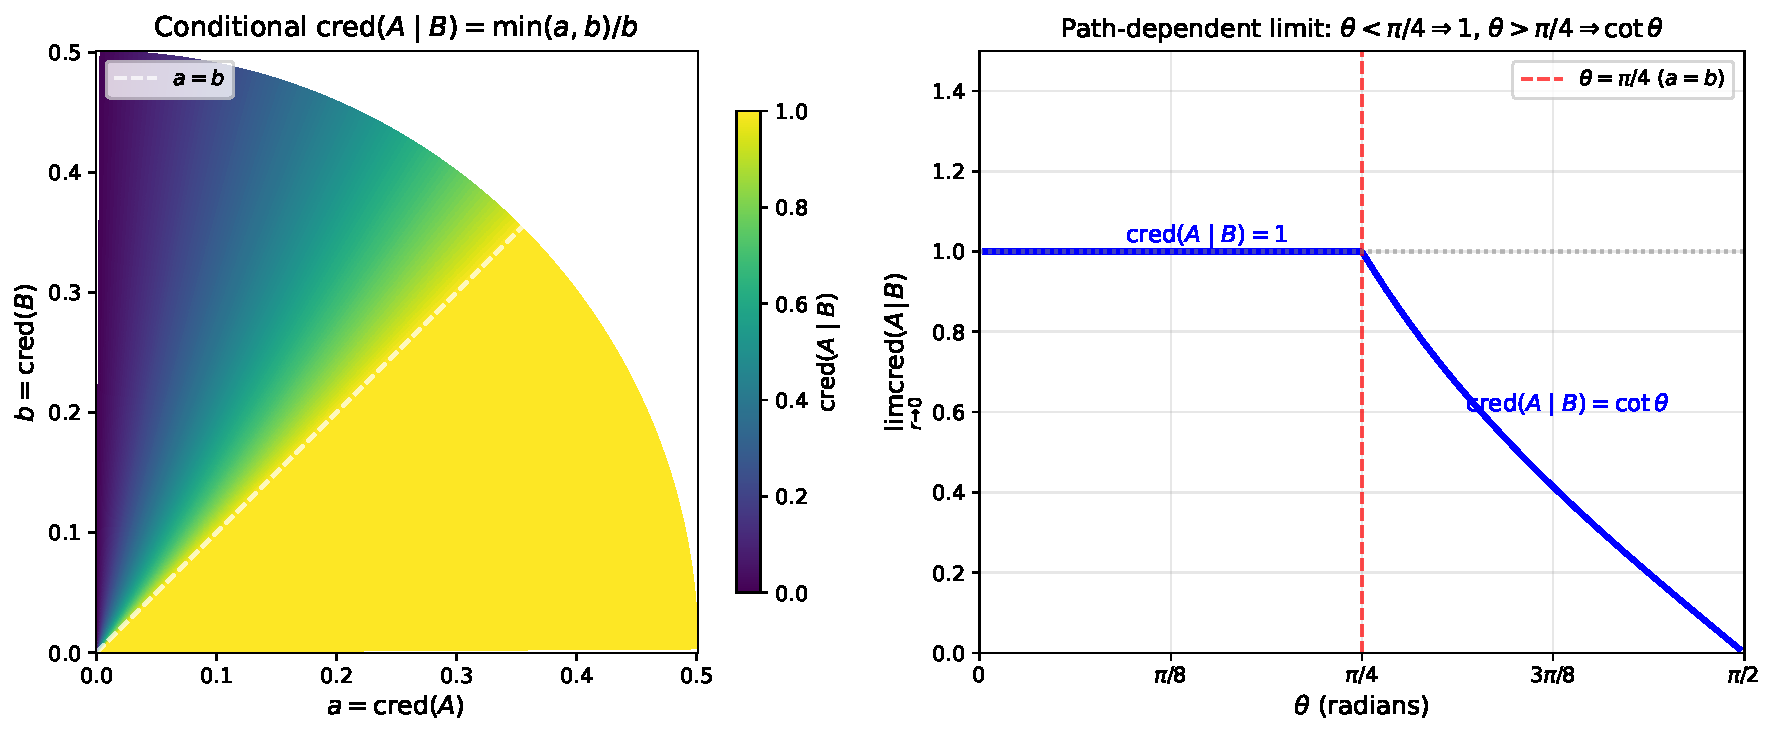
\includegraphics[width=\textwidth]{figures/path_dependence}
\caption{Path dependence at evidence zero. \textbf{Left:} Conditional $\cred(A \mid B) = \min(a,b)/b$ near the origin; value depends on angle $\theta$, not radius $r$. \textbf{Right:} Limit as $r \to 0$: equals $1$ for $\theta < \pi/4$ and $\cot\theta$ for $\theta > \pi/4$.}
\label{fig:path-dependence}
\end{figure}

\begin{remark}[Connection to the Borel--Kolmogorov Paradox]
Theorem~\ref{thm:path-dependence} has the same structure as the
\emph{Borel--Kolmogorov paradox}~\cite{borel1909,kolmogorov1933}: in measure
theory, conditioning on a null event is not uniquely determined---the ``value''
depends on the limiting procedure.
Regular conditional probabilities are defined only almost surely and may differ
on null sets.
The path dependence is the same phenomenon in algebraic form: the chain rule
does not select a unique limit at zero; it selects an angle-dependent family
of limits.
\end{remark}

The chain rule permits any value at evidence zero (Option~A: keep underdetermined, ex falso does not follow) or one can declare $\cred(A \mid 0) = 1$ (Option~B: totalize, recovering ex falso as a convention).
We take Option~A.

\subsection{De Finetti's Void}

De Finetti's three-valued conditional~\cite{definetti1936} captures the same
principle in a discrete setting: when the conditioning event does not obtain,
the conditional is void rather than vacuously true.
In the credence algebra's graded setting, ``void'' becomes ``any value in $[0,1]$ satisfies
the chain rule.''

\subsection{Existence and Uniqueness}

% Lean: conditioning_mk
\begin{theorem}[Existence]
\label{thm:existence}
If $\cred(B) > 0$ and $\cred(A \land B) \leq \cred(B)$, then there exists a
conditioning structure with $\cred(A \mid B) = \cred(A \land B)/\cred(B)$.
\end{theorem}
\begin{proof}
The value $\cred(A \land B)/\cred(B)$ lies in $[0,1]$ (by the hypotheses) and
satisfies the chain rule.
Lean: \texttt{conditioning\_mk}.
\end{proof}

% Lean: conditioning_unique
\begin{theorem}[Uniqueness of Conditioning]
\label{thm:uniqueness}
If $\cred(B) > 0$, the conditional credence is uniquely determined.
\end{theorem}
\begin{proof}
Suppose $c_1 \cdot e = c_2 \cdot e = j$ where $e = \cred(B) > 0$.
Since $e > 0$ we may cancel: $c_1 = j/e = c_2$.
Lean: \texttt{conditioning\_unique}.
\end{proof}

The condition $\cred(A \land B) \leq \cred(B)$ is both necessary and sufficient
for existence when $\cred(B) > 0$: any conditioning structure forces
$\text{joint} \leq \text{evidence}$ (since $\text{condCred} \leq 1$;
Lean: \texttt{conditioning\_implies\_joint\_le\_evidence}).
The defining constraint uses only multiplication.
Division appears in the existence proof as a construction technique, not in the
definition itself---it is derived, not primitive.
Probability satisfies the same chain rule: $P(A \mid B) \cdot P(B) = P(A \land B)$.
The credence algebra's conditioning is not new machinery---it is probability's chain rule without
the surrounding measure theory.

\subsection{Worked Example}

\begin{example}
\label{ex:conditioning}
Suppose $\cred(B) = 0.6$ and $\cred(A \land B) = 0.4$.
The joint credence is an input---it might come from empirical data, domain expertise,
or a probability model.
The chain rule gives:
\[
\cred(A \mid B) = \frac{0.4}{0.6} = \frac{2}{3}
\]
Verification: $\frac{2}{3} \cdot 0.6 = 0.4 = \cred(A \land B)$.

If instead $\cred(B) = 0$, then necessarily $\cred(A \land B) = 0$, and any
value $c \in [0,1]$ satisfies $c \cdot 0 = 0$.
The conditional is unconstrained.
\end{example}

%=============================================================================
\section{Fixed Points}
\label{sec:fixed-points}
%=============================================================================

% Lean: liar_fixed_point
\begin{theorem}[Negation Fixed Point]
\label{thm:liar}
$\negc \tfrac{1}{2} = \tfrac{1}{2}$.
\end{theorem}
\begin{proof}
$1 - \tfrac{1}{2} = \tfrac{1}{2}$.
Lean: \texttt{liar\_fixed\_point}.
\end{proof}

% Lean: neg_fixed_point_unique
\begin{theorem}[Uniqueness of Fixed Point]
\label{thm:fixedunique}
$\negc c = c$ if and only if $c = \tfrac{1}{2}$.
\end{theorem}
\begin{proof}
$1 - c = c$ implies $c = \tfrac{1}{2}$.
Lean: \texttt{neg\_fixed\_point\_unique}.
\end{proof}

If one imposes the constraint $\cred(L) = \negc \cred(L)$ for a
self-negating sentence $L$, the unique solution is $\cred(L) = \tfrac{1}{2}$.
This provides a natural algebraic value for such sentences.

\begin{remark}[Scope]
This fixed-point result is algebraic, not philosophical.
It does not resolve the liar paradox or address the strengthened liar
(``This sentence is not true'').
The extensive literature on semantic paradoxes offers multiple approaches:
Kripke's groundedness~\cite{kripke1975} assigns no truth value to the liar at
minimal fixed points; Priest's dialetheism~\cite{priest1979} treats it as both
true and false.
The credence algebra's $\tfrac{1}{2}$ is simply the unique fixed point of complement on $[0,1]$.
\end{remark}

%=============================================================================
\section{Collapse to the Kleene Lattice}
\label{sec:collapse}
%=============================================================================

Define the collapse function:
\[
\text{collapse}(c) = \begin{cases}
0 & \text{if } c = 0 \\
\tfrac{1}{2} & \text{if } 0 < c < 1 \\
1 & \text{if } c = 1
\end{cases}
\]

% Lean: collapse_neg, collapse_conj, collapse_disj, collapse_surjective
\begin{theorem}[Collapse Homomorphism]
\label{thm:collapse}
The collapse is a surjective homomorphism of the algebraic signature
$\{\negc, \conjc, \disjc\}$ from $([0,1], \negc, \conjc, \disjc)$
to the three-valued algebra $(\{0, \tfrac{1}{2}, 1\}, \mathrm{neg}, \mathrm{conj}, \mathrm{disj})$:
\begin{align*}
\mathrm{collapse}(\negc c) &= \mathrm{neg}(\mathrm{collapse}(c)) \\
\mathrm{collapse}(c_1 \conjc c_2) &= \mathrm{conj}(\mathrm{collapse}(c_1), \mathrm{collapse}(c_2)) \\
\mathrm{collapse}(c_1 \disjc c_2) &= \mathrm{disj}(\mathrm{collapse}(c_1), \mathrm{collapse}(c_2))
\end{align*}
where the three-valued operations are $\mathrm{neg}(c) = 1-c$,
$\mathrm{conj} = \min$, $\mathrm{disj} = \max$.
(The roman-font names $\mathrm{neg}$, $\mathrm{conj}$, $\mathrm{disj}$
denote the target algebra's operations; $\negc$, $\conjc$, $\disjc$
denote the credence algebra's. Both negations are $1 - c$, but the notational distinction
tracks source vs.\ target.)
\end{theorem}
\begin{proof}
We verify each operation by case analysis on whether each $c_i$ is $0$, $1$,
or in the open interval $(0,1)$.

\emph{Negation.}
If $c = 0$ then $\negc c = 1$, and $\mathrm{neg}(0) = 1$.
If $c = 1$ then $\negc c = 0$, and $\mathrm{neg}(1) = 0$.
If $0 < c < 1$ then $0 < 1 - c < 1$, so both $c$ and $\negc c$ collapse to
$\tfrac{1}{2}$, and $\mathrm{neg}(\tfrac{1}{2}) = \tfrac{1}{2}$.

\emph{Conjunction.}
If $c_1 = 0$ or $c_2 = 0$: $c_1 \conjc c_2 = 0$ (absorber), and
$\min(v_1, v_2) = 0$ whenever either $v_i = 0$.
If $c_1 = 1$: $c_1 \conjc c_2 = c_2$ (identity), and $\min(1, v_2) = v_2$.
Symmetrically for $c_2 = 1$.
The remaining case is $0 < c_1, c_2 < 1$.
Then $0 < c_1 c_2$ (product of positives) and $c_1 c_2 < c_1 \cdot 1 = c_1 < 1$
(using $c_1 > 0$ and $c_2 < 1$), so $c_1 \conjc c_2 \in (0,1)$ collapses to $\tfrac{1}{2}$,
and $\min(\tfrac{1}{2}, \tfrac{1}{2}) = \tfrac{1}{2}$.

\emph{Disjunction.}
If $c_1 = 1$ or $c_2 = 1$: $c_1 \disjc c_2 = 1$, and $\max(v_1, v_2) = 1$.
If $c_1 = 0$: $c_1 \disjc c_2 = c_2$, and $\max(0, v_2) = v_2$.
If $0 < c_1, c_2 < 1$: the disjunction is $c_1 + c_2 - c_1 c_2$.
This is positive (since $c_1 c_2 < c_1 + c_2$) and strictly less than $1$
(since $c_1 + c_2 - c_1 c_2 = 1 - (1-c_1)(1-c_2) < 1$), so it collapses to
$\tfrac{1}{2} = \max(\tfrac{1}{2}, \tfrac{1}{2})$.

Surjectivity: $\mathrm{collapse}(0) = 0$, $\mathrm{collapse}(\tfrac{1}{2}) = \tfrac{1}{2}$,
$\mathrm{collapse}(1) = 1$.

Lean: \texttt{collapse\_neg}, \texttt{collapse\_conj}, \texttt{collapse\_disj}.
\end{proof}

The three-valued algebra $(\{0, \tfrac{1}{2}, 1\}, \min, \max, 1{-}c)$ is the
\emph{Kleene lattice}: the three-element totally ordered set with
$\mathrm{conj} = \min$, $\mathrm{disj} = \max$, and involution
$\mathrm{neg}(c) = 1 - c$~\cite{kleene1952}.
It is a De Morgan lattice: a bounded distributive lattice with an
involutive order-reversing negation satisfying De Morgan's laws.
This algebra underlies three well-known logics that share the same truth tables for
negation, conjunction, and disjunction:
strong Kleene logic K$_3$~\cite{kleene1952},
Priest's Logic of Paradox LP~\cite{priest1979}, and
RM3~\cite{meyer1972}.
These logics differ only in their consequence relations---which truth values
count as ``designated'' for valid inference---not in their truth tables for
negation, conjunction, and disjunction.
K$_3$ designates only $1$; LP designates $1$ and $\tfrac{1}{2}$; RM3 designates
$1$ and $\tfrac{1}{2}$ with an additional relevance condition.
Since the credence algebra has no consequence relation, the collapse connects
it to all three simultaneously: the algebra is shared, and the choice of
consequence relation is left to whatever system is built on top.

The three-valued operations are:
\begin{center}
\begin{tabular}{c|c}
$c$ & $\mathrm{neg}(c)$ \\
\hline
0 & 1 \\
$\tfrac{1}{2}$ & $\tfrac{1}{2}$ \\
1 & 0
\end{tabular}
\quad
\begin{tabular}{c|ccc}
$\mathrm{conj}$ & 0 & $\tfrac{1}{2}$ & 1 \\
\hline
0 & 0 & 0 & 0 \\
$\tfrac{1}{2}$ & 0 & $\tfrac{1}{2}$ & $\tfrac{1}{2}$ \\
1 & 0 & $\tfrac{1}{2}$ & 1
\end{tabular}
\quad
\begin{tabular}{c|ccc}
$\mathrm{disj}$ & 0 & $\tfrac{1}{2}$ & 1 \\
\hline
0 & 0 & $\tfrac{1}{2}$ & 1 \\
$\tfrac{1}{2}$ & $\tfrac{1}{2}$ & $\tfrac{1}{2}$ & 1 \\
1 & 1 & 1 & 1
\end{tabular}
\end{center}

\subsection{Impossibility Results}

No analogous collapse exists for the other standard three-valued algebras.

% Lean: no_boolean_neg_retraction
\begin{proposition}[No Collapse to Classical Logic]
\label{prop:no-classical}
There is no function $\varphi : [0,1] \to \{0,1\}$ preserving negation:
$\varphi(1-c) = 1 - \varphi(c)$ for all $c$.
\end{proposition}
\begin{proof}
At $c = \tfrac{1}{2}$: $\varphi(\tfrac{1}{2}) = 1 - \varphi(\tfrac{1}{2})$,
so $\varphi(\tfrac{1}{2}) = \tfrac{1}{2} \notin \{0, 1\}$.
Lean: \texttt{no\_boolean\_neg\_retraction}.
\end{proof}

% Lean: no_godel_collapse, godel_neg_no_fixed_point
\begin{proposition}[No Collapse to G\"odel Logic]
\label{prop:no-godel}
Let $\mathrm{neg}_G$ denote G\"odel negation on $\{0, \tfrac{1}{2}, 1\}$:
$\mathrm{neg}_G(0) = 1$ and $\mathrm{neg}_G(c) = 0$ for $c > 0$~\cite{godel1932}.
There is no function $\varphi : [0,1] \to \{0, \tfrac{1}{2}, 1\}$ such that
$\varphi(1-c) = \mathrm{neg}_G(\varphi(c))$ for all $c$.
\end{proposition}
\begin{proof}
G\"odel negation has no fixed point:
$\mathrm{neg}_G(0) = 1 \neq 0$,
$\mathrm{neg}_G(\tfrac{1}{2}) = 0 \neq \tfrac{1}{2}$,
$\mathrm{neg}_G(1) = 0 \neq 1$.
But $\varphi(\tfrac{1}{2}) = \varphi(1 - \tfrac{1}{2}) = \mathrm{neg}_G(\varphi(\tfrac{1}{2}))$
requires $\varphi(\tfrac{1}{2})$ to be a fixed point.
Lean: \texttt{no\_godel\_collapse}, \texttt{godel\_neg\_no\_fixed\_point}.
\end{proof}

% Lean: no_luk_collapse, luk_conj_half_half
\begin{proposition}[No Collapse to \L ukasiewicz Logic]
\label{prop:no-luk}
Let $\mathrm{conj}_{\text{\L}} (a, b) = \max(a + b - 1,\; 0)$ be the \L ukasiewicz
conjunction on $\{0, \tfrac{1}{2}, 1\}$~\cite{lukasiewicz1920}.
There is no function $\varphi : [0,1] \to \{0, \tfrac{1}{2}, 1\}$ preserving both
negation ($\varphi(1-c) = 1-\varphi(c)$) and conjunction
($\varphi(c_1 \cdot c_2) = \mathrm{conj}_{\text{\L}}(\varphi(c_1), \varphi(c_2))$).
\end{proposition}
\begin{proof}
Negation preservation at $c = \tfrac{1}{2}$:
$\varphi(\tfrac{1}{2}) = \varphi(1 - \tfrac{1}{2}) = 1 - \varphi(\tfrac{1}{2})$,
so $\varphi(\tfrac{1}{2}) = \tfrac{1}{2}$.
Pick $c = \sqrt{1/2}$; since $0 < \sqrt{1/2} < 1$, we have $c \in (0,1)$,
and $c \conjc c = c^2 = \tfrac{1}{2}$.
Conjunction preservation gives
$\varphi(\tfrac{1}{2}) = \mathrm{conj}_{\text{\L}}(\varphi(c), \varphi(c))$.
Since $\varphi(c) \in \{0, \tfrac{1}{2}, 1\}$:
\[
\mathrm{conj}_{\text{\L}}(0,0) = 0,\quad
\mathrm{conj}_{\text{\L}}(\tfrac{1}{2},\tfrac{1}{2}) = 0,\quad
\mathrm{conj}_{\text{\L}}(1,1) = 1
\]
None equals $\tfrac{1}{2} = \varphi(\tfrac{1}{2})$.
Lean: \texttt{no\_luk\_collapse}, \texttt{luk\_conj\_half\_half}.
\end{proof}

The pattern: the negation fixed point at $\tfrac{1}{2}$ propagates constraints
that only the Kleene lattice can absorb.
Classical logic and G\"odel logic fail on negation alone (they lack a fixed
point).
\L ukasiewicz logic preserves negation, but its conjunction
$\mathrm{conj}_{\text{\L}}(\tfrac{1}{2}, \tfrac{1}{2}) = 0$ disagrees with the
Kleene value $\min(\tfrac{1}{2}, \tfrac{1}{2}) = \tfrac{1}{2}$: the
self-conjunction of the fixed point must equal the fixed point, and only the
Kleene lattice satisfies this.
See Appendix~\ref{app:extended} for the Belnap-Dunn comparison.

%=============================================================================
\section{Relationship to Existing Frameworks}
\label{sec:relationships}
%=============================================================================

\subsection{Conditioning and Implication}

The homomorphism of Theorem~\ref{thm:collapse} covers $\{\negc, \conjc, \disjc\}$.
Implication is a separate question: the Kleene lattice has no canonical arrow,
and the three logics (K$_3$, LP, RM3) that share it each define implication
differently.

Chain-rule conditioning involves three quantities: evidence, joint, and the
conditional credence.
For evidence $> 0$, the conditional is $\text{joint}/\text{evidence}$, which
requires joint $\leq$ evidence.
To compare with standard binary implications, fix the joint to the Kleene conjunction
$\min(a, b)$.
For evidence $a > 0$, the chain rule gives
$\text{cond}(a, b) = \min(a, b)/a = \min(b/a,\; 1)$---exactly the \emph{product residuated implication} of H\'ajek's
$\Pi$-logic~\cite{hajek1998}.

\textbf{Three-way comparison on $\{0, \tfrac{1}{2}, 1\}$.}

\begin{center}
\begin{tabular}{c|ccc}
\multicolumn{4}{c}{\textbf{Kleene material}\footnotemark\ (Lean: \texttt{rm3\_impl}): $\max(\negc a, b)$} \\
& 0 & $\tfrac{1}{2}$ & 1 \\
\hline
0 & 1 & 1 & 1 \\
$\tfrac{1}{2}$ & $\tfrac{1}{2}$ & $\tfrac{1}{2}$ & 1 \\
1 & 0 & $\tfrac{1}{2}$ & 1
\end{tabular}
\quad
\begin{tabular}{c|ccc}
\multicolumn{4}{c}{\textbf{Prod.\ resid.\ / G\"odel}\footnotemark: $\min(b/a, 1)$} \\
& 0 & $\tfrac{1}{2}$ & 1 \\
\hline
0 & 1 & 1 & 1 \\
$\tfrac{1}{2}$ & 0 & 1 & 1 \\
1 & 0 & $\tfrac{1}{2}$ & 1
\end{tabular}
\quad
\begin{tabular}{c|ccc}
\multicolumn{4}{c}{\textbf{Chain-rule}: joint $= \min(a,b)$} \\
& 0 & $\tfrac{1}{2}$ & 1 \\
\hline
0 & $*$ & $*$ & $*$ \\
$\tfrac{1}{2}$ & 0 & 1 & 1 \\
1 & 0 & $\tfrac{1}{2}$ & 1
\end{tabular}
\end{center}
\smallskip
{\footnotesize $*$ = unconstrained. Rows with evidence $> 0$ are uniquely
determined. The product residuated and chain-rule tables agree everywhere except
the evidence $= 0$ row.}

\footnotetext{The Kleene material conditional $\max(\negc a, b)$ is the
truth-functional arrow shared by K$_3$, LP, and
RM3~\cite[Table~7.3.3]{priest2008}. We use the term ``Kleene material''
to emphasize that it is a connective on the Kleene lattice, not specific
to any one logic's consequence relation.}
\footnotetext{On $\{0, \tfrac{1}{2}, 1\}$, the product residuated implication
$\min(b/a, 1)$ coincides with the G\"odel implication.
Lean: \texttt{godel\_impl\_eq\_prod\_resid}.}

Lean: \texttt{rm3\_impl}, \texttt{godel\_impl},
\texttt{godel\_impl\_ne\_rm3\_impl}, \texttt{cred\_no\_ex\_falso\_godel}.

\subsection{Bayes Consistency}

Applying the chain rule from both directions gives Bayes' theorem:
\[
\cred(A \mid B) \cdot \cred(B) = \cred(A \land B) = \cred(B \land A) = \cred(B \mid A) \cdot \cred(A).
\]
\begin{definition}[Bayes Consistency]
\label{def:bayes}
A binary arrow $f : [0,1]^2 \to [0,1]$ is
\emph{Bayes-consistent} when the joint it induces is symmetric:
$f(a, b) \cdot a = f(b, a) \cdot b$ for all $a, b \in [0,1]$.
\end{definition}

% Lean: prod_resid_bayes_consistent_real
\begin{proposition}[Product Residuated is Bayes-Consistent]
\label{prop:resid-bayes}
The product residuated implication $f(a, b) = \min(b/a,\; 1)$ (with
the standard convention $f(0, b) = 1$) is
Bayes-consistent: $f(a, b) \cdot a = \min(a, b) = f(b, a) \cdot b$.
\end{proposition}
\begin{proof}
If $a = 0$: $f(0, b) \cdot 0 = 0 = \min(0, b)$, and symmetrically
$f(b, 0) \cdot b = 0$ (since $f(b, 0) = \min(0/b, 1) = 0$ for $b > 0$,
and $f(0, 0) \cdot 0 = 0$).
If $a > 0$ and $b \leq a$: $f(a, b) \cdot a = (b/a) \cdot a = b = \min(a, b)$.
If $a > 0$ and $a < b$: $f(a, b) \cdot a = 1 \cdot a = a = \min(a, b)$.
Lean: \texttt{prod\_resid\_bayes\_consistent\_real}.
\end{proof}

% Lean: godel_not_bayes_consistent_real
\begin{proposition}[G\"odel is Not Bayes-Consistent on the Continuum]
\label{prop:godel-not-bayes}
The G\"odel implication ($f(a,b) = 1$ if $a \leq b$, else $b$) fails
Bayes consistency on $[0,1]$.
\end{proposition}
\begin{proof}
Take $a = \tfrac{2}{5}$, $b = \tfrac{3}{5}$.
Then $f(a, b) = 1$ (since $a \leq b$), so $f(a, b) \cdot a = \tfrac{2}{5}$.
But $f(b, a) = a = \tfrac{2}{5}$ (since $b > a$), so
$f(b, a) \cdot b = \tfrac{2}{5} \cdot \tfrac{3}{5} = \tfrac{6}{25} \neq \tfrac{2}{5}$.
Lean: \texttt{godel\_not\_bayes\_consistent\_real}.
\end{proof}

% Lean: rm3_not_bayes_consistent_real
\begin{proposition}[RM3 is Not Bayes-Consistent]
\label{prop:rm3-not-bayes}
The Kleene material conditional $\max(\negc a, b)$ fails
Bayes consistency even on $\{0, \tfrac{1}{2}, 1\}$.
\end{proposition}
\begin{proof}
Take $a = \tfrac{1}{2}$, $b = 0$.
Then $f(a, b) = \max(\tfrac{1}{2}, 0) = \tfrac{1}{2}$, so
$f(a, b) \cdot a = \tfrac{1}{4}$.
But $f(b, a) = \max(1, \tfrac{1}{2}) = 1$, so $f(b, a) \cdot b = 0$.
Since $\tfrac{1}{4} \neq 0$, RM3 is not Bayes-consistent.
Lean: \texttt{rm3\_not\_bayes\_consistent\_real}.
\end{proof}

\begin{center}
\small
\begin{tabular}{lcccc}
\toprule
\textbf{Joint formula} & \textbf{Truth-func.} & \textbf{Bayes-cons.} & \textbf{Non-trivial} & \textbf{Idempotent} \\
\midrule
$\min(a,b)$ (max.\ pos.\ dep.) & \checkmark & \checkmark & \checkmark & \checkmark \\
$a \cdot b$ (independence) & \checkmark & \checkmark & $\times$ & $\times$ \\
$\max(a+b-1,0)$ (\L uk.) & \checkmark & \checkmark & \checkmark & $\times$ \\
RM3 induced & --- & $\times$ & --- & --- \\
G\"odel induced (on $[0,1]$) & --- & $\times$ & --- & --- \\
External (probability) & $\times$ & \checkmark & \checkmark & \checkmark \\
\bottomrule
\end{tabular}
\normalsize
\captionof{table}{Comparison of joint formulas.
Only the minimum (Fr\'echet upper bound) satisfies all four requirements for
logic-style reasoning.
External joints (probability-style) satisfy all except truth-functionality.}
\label{tab:joint-comparison}
\end{center}

\subsection{Relationship to Probability}
\label{sec:probability}

Every probability space satisfies the credence algebra's axioms, making probability a special case.
In logic, the algebra is uninterpreted; a valuation and consequence relation are separate layers.
In probability, algebra and semantics are fused: the Kolmogorov axioms define $P$ on events,
and the chain rule is simultaneously algebraic and semantic.
The credence algebra stays on the logic side of this divide
(Remark~\ref{rem:algebraic-conditioning}): its chain rule constrains three numbers
with no reference to propositions or a measure.

What probability adds: a sigma-algebra of events, a countably additive measure determining the joint $P(A \land B)$, and sigma-additivity.
What the algebra drops: no measure, no sigma-algebra, no additivity, no event structure, no consequence relation.
At evidence zero, probability is undefined; the credence algebra is unconstrained.

\begin{center}
\small
\begin{tabular}{llp{3.5cm}l}
\toprule
\textbf{System} & \textbf{Layer} & \textbf{Core axioms} & \textbf{At evidence $= 0$} \\
\midrule
\textbf{Credence algebra} & Constraint algebra & $[0,1]$ + complement + chain rule & Unconstrained$^{**}$ \\
Probability & Semantic system & Chain rule + measure + $\sigma$-additivity & Undefined$^*$ \\
Product fuzzy ($\Pi$) & Deductive system & $[0,1]$ + product + residuated impl. & $0 \to y = 1$ \\
Classical logic & Deductive system & $\{0,1\}$ + Boolean ops + material impl. & $0 \to y = 1$ \\
RM3 & Deductive system & $\{0,\tfrac{1}{2},1\}$ + De Morgan + $\max$ impl. & $0 \to y = 1$$^\dagger$ \\
\bottomrule
\end{tabular}
\normalsize
\end{center}
\smallskip
\noindent {\footnotesize $^*$Undefined: $P(A \mid B) = P(A \land B)/P(B)$ is ill-formed. \quad
$^{**}$Unconstrained: $c \cdot 0 = 0$ holds for every $c \in [0,1]$. \quad
$^\dagger$RM3 has $0 \to b = 1$ in its truth table but blocks explosion at the consequence-relation level.}

\subsection{Related Work}
\label{sec:related}

The credence algebra sits in a web of prior work.
The hierarchy---the credence algebra as a weakening of probability, distinct from product fuzzy
logic---organizes the relationships.

\textbf{Primitive Conditional Probability.}
R\'enyi~\cite{renyi1955,renyi1970} first axiomatized conditional probability as
primitive, with the chain rule as a defining constraint rather than division.
Popper~\cite{popper1959} independently argued that conditional probability is more
fundamental than absolute probability, developing ``Popper functions.''
Van Fraassen~\cite{vanfraassen1976} extended the Popper-R\'enyi approach.
The credence algebra inherits the chain rule from this tradition but drops the measure space
entirely.

\textbf{Conditional Events.}
De Finetti's three-valued conditional~\cite{definetti1936}---true when
$A \land B$, false when $\lnot A \land B$, void when $\lnot B$---is
the credence algebra's unconstrained conditioning applied in a discrete setting
(Section~\ref{sec:intro}).
Calabrese~\cite{calabrese1987} formalized conditional events as ``Boolean
fractions'' with three-valued indicator functions.
\'Egr\'e, Rossi, and Sprenger~\cite{egre2021} showed that
de Finetti's conditional, combined with Kleene's strong
connectives, produces logics in which explosion fails at the semantic
level---not via a consequence relation but via the truth table itself.
Relevant logics (RM3, R, E) and paraconsistent logics (LP) block explosion
at the \emph{consequence-relation} level: RM3 has $0 \to b = 1$ in its truth
table but restricts which inferences are valid~\cite{priest2008}.
De Finetti's approach and the credence algebra block it at the \emph{algebraic} level: the
conditional is void or unconstrained when the antecedent fails, so the
truth table itself never forces $0 \to b = 1$.

\textbf{Probability and Relevant Logic.}
Van Fraassen~\cite{vanfraassen1983} showed that conditional probability functions
can model relevant logic's consequence relation, connecting probabilistic and
relevance-based approaches.
The credence algebra makes this connection algebraically explicit through the collapse homomorphism.

\textbf{Product Fuzzy Logic.}
H\'ajek~\cite{hajek1998} developed product logic ($\Pi$), which uses the product
t-norm with \emph{residuated} implication ($x \to y = \min(y/x, 1)$ for $x > 0$,
and $0 \to y = 1$); the residuated implication forces ex falso.
Klement, Mesiar, and Pap~\cite{klement2000} gave a comprehensive treatment of
triangular norms; the product t-norm, probabilistic sum, and standard complement
form the product De Morgan triplet.
Goguen~\cite{goguen1969} introduced the product t-norm as a conjunction for
inexact concepts; Esteva et al.~\cite{esteva2000} showed that extending product
logic with an involutive negation yields exactly the connective algebra adopted here
(product t-norm, probabilistic sum, standard complement).
The credence algebra shares this triplet and, when conditioning is instantiated with the Kleene
joint $\min(a, b)$, \emph{recovers} the product residuated implication for
evidence $> 0$.
The divergence is solely at evidence $= 0$: product logic forces $0 \to y = 1$;
chain-rule conditioning is unconstrained.
On the finite set $\{0, \tfrac{1}{2}, 1\}$, the product residuated implication
coincides with the G\"odel implication; on $[0,1]$ they diverge.

\textbf{Fuzzy Logic and Conditional Probability.}
H\'ajek, Godo, and Esteva~\cite{hajek1995} studied conditional probability
within fuzzy logic and noted that the product residuated implication is
discontinuous.
As a workaround, they expressed $P(\psi \mid \varphi) \geq a$ via the
chain rule constraint $P(\varphi \land \psi) \geq a \cdot P(\varphi)$
rather than division---essentially the same move the credence algebra makes.
They treated this as a technical device; the algebra adopts it as the defining
design choice and explores its algebraic consequences.

\textbf{Cox-Jaynes Probability Logic.}
Cox's theorem~\cite{cox1961} proves that any consistent system for plausible
reasoning satisfying certain desiderata must be isomorphic to probability theory.
Jaynes~\cite{jaynes2003} developed this into ``Probability Theory: The Logic of
Science.''
Cox's desiderata require conditioning to be a \emph{function} (unique output for
each input). The credence algebra relaxes this: conditioning is a \emph{relation} that becomes
non-functional when evidence $= 0$.

\textbf{Conditionals and Triviality.}
Adams~\cite{adams1965,adams1998} developed probabilistic semantics for conditionals
where $P(A \to B) = P(B|A)$.
Lewis~\cite{lewis1976} proved that treating conditionals as propositions with this
property leads to triviality.
The credence algebra sidesteps triviality by treating conditioning as a structural operation,
not as a credence assigned to a conditional proposition.

\textbf{Relevant and Paraconsistent Logic.}
Anderson and Belnap~\cite{anderson1975} developed relevant logics R and E,
rejecting ex falso via syntactic relevance conditions.
Dunn~\cite{dunn1976} provided algebraic semantics connecting relevant logic to
De Morgan lattices.
RM3~\cite{meyer1972} is a three-valued relevant logic.
Da Costa~\cite{dacosta1974} developed paraconsistent logics tolerating contradiction
without explosion.
Priest~\cite{priest1979} introduced the Logic of Paradox (LP).
Brady~\cite{brady2006} and Weber~\cite{weber2010} developed paraconsistent set
theory with unrestricted comprehension.
The collapse homomorphism (Section~\ref{sec:collapse}) connects the credence algebra to the
Kleene lattice~\cite{kleene1952} that underlies K$_3$, LP, and RM3.
These three logics share the same truth tables for $\{\negc, \conjc, \disjc\}$;
the collapse is to this shared algebra, not to any one logic's consequence relation.

\textbf{Many-Valued Logics.}
\L ukasiewicz~\cite{lukasiewicz1920} introduced three-valued and infinite-valued logics.
Kleene~\cite{kleene1952} developed strong and weak three-valued logics.
G\"odel~\cite{godel1932} introduced three-valued intuitionistic logic.
Belnap~\cite{belnap1977} introduced a four-valued logic for reasoning with
incomplete and contradictory information.
Zadeh~\cite{zadeh1965} introduced fuzzy sets with $[0,1]$ membership degrees.
Section~\ref{sec:scope} shows that no analogous collapse exists for
\L ukasiewicz, G\"odel, or classical algebras, making the Kleene lattice the only standard three-valued quotient of the credence algebra.
Ferm\"uller~\cite{fermuller2014} reached the same conclusion from game
semantics (Main Theorem): straightforward generalizations of Hintikka's
evaluation game yield Kleene logic and nothing stronger.

\textbf{Copulas and Fuzzy Implications.}
Grzegorzewski~\cite{grzegorzewski2013} defined \emph{probabilistic
implications} $I_C(a,b) = C(a,b)/a$ from a copula $C$ and computed that
the Fr\'echet upper bound (min copula) yields the Goguen~\cite{goguen1969} (product
residuated) implication.
This is the copula-side construction; the credence algebra arrives at the same arrow from
the chain-rule side by setting joint $= \min(a,b)$.
The Bayes consistency criterion---that $f(a,b) \cdot a = f(b,a) \cdot b$,
equivalently that the induced joint is symmetric---and its use as a
diagnostic lens for why RM3 and G\"odel arrows fail in the present setting
(they are not copula-derived) is, to our knowledge, not standard in the
relevant-logic literature.

\textbf{Measure-Theoretic Conditioning.}
In measure theory, conditioning on null sets uses disintegration~\cite{chang1997},
yielding a specific (a.e.\ unique) value determined by the measure structure.
Fritz~\cite{fritz2020} treats conditioning categorically via Markov categories.
The credence algebra drops the measure, so disintegration does not apply; at evidence zero, the
conditional is unconstrained rather than determined.

\textbf{The credence algebra's contributions.}
The product De Morgan triplet is standard~\cite{klement2000}; product logic
with involutive negation was studied by Esteva et al.~\cite{esteva2000};
primitive conditioning is due to
R\'enyi and Popper; void conditionals at the algebraic level are due to
de Finetti; the algebraic formalization of conditional events is due to
Calabrese; the connection to relevant logic is van Fraassen's;
the chain rule constraint in a fuzzy setting appears in H\'ajek et al.;
copula-derived implications are due to Grzegorzewski.
Given this prior art, the credence algebra contributes:
\begin{enumerate}[label=(\arabic*)]
\item Identifying the chain rule as the sole structural axiom needed beyond
$[0,1]$ and complement---a weakening of probability that retains conditioning
while dropping the measure.
\item Chain-rule conditioning in the product De Morgan triplet, continuing
de Finetti's void-conditional tradition~\cite{definetti1936} in a graded
setting.
H\'ajek et al.~\cite{hajek1995} used the chain rule constraint as a
technical device; the algebra adopts it as the defining structural axiom.
\item The explicit collapse homomorphism to the Kleene lattice (underlying
K$_3$, LP, and RM3), with impossibility results for \L ukasiewicz, G\"odel,
and classical targets, and Lean verification.
\item Bayes consistency as a selection criterion: the product residuated
implication passes; RM3 and G\"odel fail.  Every symmetric copula yields
a Bayes-consistent arrow (machine-checked on three values and on $[0,1]$).
\item Systematic treatment of fixed points with machine-checked proofs.
\end{enumerate}

%=============================================================================
% Lean section moved to Appendix C
% See \ref{app:lean} for details
%=============================================================================

%=============================================================================
\section{Conclusion}
\label{sec:conclusion}
%=============================================================================

Theorem~\ref{thm:uniqueness-main} shows the min conjunction is forced by
Bayes consistency, non-triviality, and idempotence.
Theorem~\ref{thm:path-dependence} shows conditioning at evidence zero is
path-dependent, so ex falso requires a convention beyond the chain rule.
Theorem~\ref{thm:collapse} provides a collapse to Kleene; Propositions
\ref{prop:no-godel}--\ref{prop:no-luk} block alternatives.

The credence algebra provides values and operations without fixing a consequence
relation or update rule.
Probability adds measure theory; product logic commits to residuation;
K$_3$/LP/RM3 choose designated values.

On the Kleene quotient, the algebra handles self-reference and undefinedness
without explosion.
On $[0,1]$, it supports Bayesian inference under comonotonicity (nested
events, single latent variable).

Part~2~\cite{part2} develops valuations, consequence relations, and update
rules.
Open problems: first-order extension, consequence relations compatible with
unconstrained conditioning at zero, connections to paraconsistent set theory.

\section*{Acknowledgements}

The author thanks Graham Priest for correspondence that clarified the
distinction between connectives and consequence relations in the context of
an earlier approach to this problem.

%=============================================================================
% Bibliography
%=============================================================================

\begin{thebibliography}{99}

\bibitem{adams1965}
Adams, E.W.
\newblock The logic of conditionals.
\newblock \emph{Inquiry}, 8:166--197, 1965.

\bibitem{adams1998}
Adams, E.W.
\newblock \emph{A Primer of Probability Logic}.
\newblock CSLI Publications, Stanford, 1998.

\bibitem{anderson1975}
Anderson, A.R. and Belnap, N.D.
\newblock \emph{Entailment: The Logic of Relevance and Necessity}, Vol.~I.
\newblock Princeton University Press, 1975.

\bibitem{belnap1977}
Belnap, N.D.
\newblock A useful four-valued logic.
\newblock In Dunn, J.M. and Epstein, G., editors, \emph{Modern Uses of
Multiple-Valued Logic}, pages 5--37. Reidel, 1977.

\bibitem{borel1909}
Borel, \'E.
\newblock \emph{\'El\'ements de la th\'eorie des probabilit\'es}.
\newblock Hermann, Paris, 1909.

\bibitem{brady2006}
Brady, R.
\newblock \emph{Universal Logic}.
\newblock CSLI Lecture Notes, vol.~109. CSLI Publications, 2006.

\bibitem{calabrese1987}
Calabrese, P.G.
\newblock An algebraic synthesis of the foundations of logic and probability.
\newblock \emph{Information Sciences}, 42:187--237, 1987.

\bibitem{carnap1950}
Carnap, R.
\newblock \emph{Logical Foundations of Probability}.
\newblock University of Chicago Press, 1950.

\bibitem{chang1997}
Chang, J.T. and Pollard, D.
\newblock Conditioning as disintegration.
\newblock \emph{Statistica Neerlandica}, 51(3):287--317, 1997.

\bibitem{cox1961}
Cox, R.T.
\newblock \emph{The Algebra of Probable Inference}.
\newblock Johns Hopkins University Press, 1961.

\bibitem{dacosta1974}
da Costa, N.C.A.
\newblock On the theory of inconsistent formal systems.
\newblock \emph{Notre Dame Journal of Formal Logic}, 15(4):497--510, 1974.

\bibitem{definetti1936}
de Finetti, B.
\newblock La logique de la probabilit\'e.
\newblock In \emph{Actes du Congr\`es International de Philosophie Scientifique},
vol.~IV, pages 1--9. Hermann, 1936.

\bibitem{definetti1937}
de Finetti, B.
\newblock La pr\'evision: ses lois logiques, ses sources subjectives.
\newblock \emph{Annales de l'Institut Henri Poincar\'e}, 7:1--68, 1937.

\bibitem{dhaene2002}
Dhaene, J., Denuit, M., Goovaerts, M.J., Kaas, R., and Vyncke, D.
\newblock The concept of comonotonicity in actuarial science and finance: Theory.
\newblock \emph{Insurance: Mathematics and Economics}, 31(1):3--33, 2002.

\bibitem{dubois2001}
Dubois, D. and Prade, H.
\newblock Possibility theory, probability theory and multiple-valued logics:
A clarification.
\newblock \emph{Annals of Mathematics and Artificial Intelligence}, 32:35--66,
2001.

\bibitem{dunn1976}
Dunn, J.M.
\newblock Intuitive semantics for first-degree entailments and coupled trees.
\newblock \emph{Philosophical Studies}, 29:149--168, 1976.

\bibitem{edgington1997}
Edgington, D.
\newblock Vagueness by degrees.
\newblock In Keefe, R. and Smith, P., editors, \emph{Vagueness: A Reader},
pages 294--316. MIT Press, 1997.

\bibitem{egre2021}
\'Egr\'e, P., Rossi, L., and Sprenger, J.
\newblock De Finettian logics of indicative conditionals, Part~I:
Trivalent semantics and validity.
\newblock \emph{Journal of Philosophical Logic}, 50:187--213, 2021.

\bibitem{esteva2000}
Esteva, F., Godo, L., H\'ajek, P., and Navara, M.
\newblock Residuated fuzzy logics with an involutive negation.
\newblock \emph{Archive for Mathematical Logic}, 39(2):103--124, 2000.

\bibitem{fermuller2014}
Ferm\"uller, C.G.
\newblock Hintikka-style semantic games for fuzzy logics.
\newblock In Beierle, C. and Meghini, C., editors, \emph{Foundations of
Information and Knowledge Systems (FoIKS 2014)}, LNCS 8367, pages 193--210.
Springer, 2014.

\bibitem{fritz2020}
Fritz, T.
\newblock A synthetic approach to Markov kernels, conditional independence
and theorems on sufficient statistics.
\newblock \emph{Advances in Mathematics}, 370, Article 107239, 2020.

\bibitem{goguen1969}
Goguen, J.A.
\newblock The logic of inexact concepts.
\newblock \emph{Synthese}, 19(3--4):325--373, 1969.

\bibitem{godel1932}
G\"odel, K.
\newblock Zum intuitionistischen Aussagenkalk\"ul.
\newblock \emph{Anzeiger der Akademie der Wissenschaften in Wien},
69:65--66, 1932.

\bibitem{grzegorzewski2013}
Grzegorzewski, P.
\newblock Probabilistic implications.
\newblock \emph{Fuzzy Sets and Systems}, 226:53--66, 2013.

\bibitem{hajek1995}
H\'ajek, P., Godo, L., and Esteva, F.
\newblock Fuzzy logic and probability.
\newblock In \emph{Proceedings of the 11th Conference on Uncertainty in
Artificial Intelligence (UAI)}, pages 237--244, 1995.

\bibitem{hajek1998}
H\'ajek, P.
\newblock \emph{Metamathematics of Fuzzy Logic}.
\newblock Trends in Logic, vol.~4. Kluwer, 1998.

\bibitem{gottwald2001}
Gottwald, S.
\newblock \emph{A Treatise on Many-Valued Logics}.
\newblock Studies in Logic and Computation, vol.~9. Research Studies Press, 2001.

\bibitem{jaynes2003}
Jaynes, E.T.
\newblock \emph{Probability Theory: The Logic of Science}.
\newblock Cambridge University Press, 2003.

\bibitem{jeffrey1965}
Jeffrey, R.C.
\newblock \emph{The Logic of Decision}.
\newblock McGraw-Hill, 1965.

\bibitem{kleene1952}
Kleene, S.C.
\newblock \emph{Introduction to Metamathematics}.
\newblock North-Holland, 1952.

\bibitem{klement2000}
Klement, E.P., Mesiar, R., and Pap, E.
\newblock \emph{Triangular Norms}.
\newblock Trends in Logic, vol.~8. Kluwer, 2000.

\bibitem{kolmogorov1933}
Kolmogorov, A.N.
\newblock \emph{Grundbegriffe der Wahrscheinlichkeitsrechnung}.
\newblock Ergebnisse der Mathematik. Springer, 1933.
\newblock English translation: \emph{Foundations of the Theory of Probability},
Chelsea, 1956.

\bibitem{kripke1975}
Kripke, S.
\newblock Outline of a theory of truth.
\newblock \emph{Journal of Philosophy}, 72(19):690--716, 1975.

\bibitem{lawvere1973}
Lawvere, F.W.
\newblock Metric spaces, generalized logic, and closed categories.
\newblock \emph{Rendiconti del Seminario Matematico e Fisico di Milano},
43:135--166, 1973.

\bibitem{lewis1976}
Lewis, D.
\newblock Probabilities of conditionals and conditional probabilities.
\newblock \emph{Philosophical Review}, 85:297--315, 1976.

\bibitem{lukasiewicz1920}
\L ukasiewicz, J.
\newblock O logice tr\'ojwarto\'sciowej.
\newblock \emph{Ruch Filozoficzny}, 5:170--171, 1920.

\bibitem{meyer1972}
Meyer, R.K. and Routley, R.
\newblock Algebraic analysis of entailment I.
\newblock \emph{Logique et Analyse}, 15:407--428, 1972.

\bibitem{nelsen2006}
Nelsen, R.B.
\newblock \emph{An Introduction to Copulas}.
\newblock Springer Series in Statistics, 2nd edition. Springer, 2006.

\bibitem{part2}
Anonymous.
\newblock Part~2: Two views of credence reasoning.
\newblock Working paper, 2026.

\bibitem{popper1959}
Popper, K.
\newblock \emph{The Logic of Scientific Discovery}.
\newblock Hutchinson, 1959.

\bibitem{panti1995}
Panti, G.
\newblock Multi-valued logics.
\newblock In Gabbay, D.M. et al., editors, \emph{Quantifiers: Logics, Models
and Computation}, volume~1, pages 27--74. Kluwer, 1995.

\bibitem{priest1979}
Priest, G.
\newblock The logic of paradox.
\newblock \emph{Journal of Philosophical Logic}, 8:219--241, 1979.

\bibitem{priest2008}
Priest, G.
\newblock \emph{An Introduction to Non-Classical Logic: From If to Is}.
\newblock Cambridge University Press, 2nd edition, 2008.

\bibitem{ramsey1931}
Ramsey, F.P.
\newblock Truth and probability.
\newblock In Braithwaite, R.B., editor, \emph{The Foundations of Mathematics
and other Logical Essays}, pages 156--198. Kegan Paul, 1931.

\bibitem{reichenbach1949}
Reichenbach, H.
\newblock \emph{The Theory of Probability}.
\newblock University of California Press, 1949.

\bibitem{renyi1955}
R\'enyi, A.
\newblock On a new axiomatic theory of probability.
\newblock \emph{Acta Mathematica Academiae Scientiarum Hungaricae}, 6:285--335, 1955.

\bibitem{renyi1970}
R\'enyi, A.
\newblock \emph{Foundations of Probability}.
\newblock Holden-Day, 1970.

\bibitem{sep-logic-probability}
H\'ajek, A.
\newblock Logic and probability.
\newblock In Zalta, E.N., editor, \emph{Stanford Encyclopedia of Philosophy}.
\newblock Stanford University, 2001; revised 2019.
\newblock \url{https://plato.stanford.edu/entries/logic-probability/}.

\bibitem{sep-reichenbach}
Glymour, C. and Eberhardt, F.
\newblock Hans Reichenbach.
\newblock In Zalta, E.N., editor, \emph{Stanford Encyclopedia of Philosophy}.
\newblock Stanford University, 2008; revised 2016.
\newblock \url{https://plato.stanford.edu/entries/reichenbach/}.

\bibitem{shafer1976}
Shafer, G.
\newblock \emph{A Mathematical Theory of Evidence}.
\newblock Princeton University Press, 1976.

\bibitem{sklar1959}
Sklar, A.
\newblock Fonctions de r\'epartition \`a $n$ dimensions et leurs marges.
\newblock \emph{Publications de l'Institut de Statistique de l'Universit\'e de Paris}, 8:229--231, 1959.

\bibitem{vanfraassen1976}
van Fraassen, B.C.
\newblock Probabilities of conditionals.
\newblock In Harper, W.L. and Hooker, C.A., editors, \emph{Foundations of
Probability Theory, Statistical Inference, and Statistical Theories of
Science}, Vol.~1, pages 261--308. Reidel, 1976.

\bibitem{vanfraassen1983}
van Fraassen, B.C.
\newblock Gentlemen's wagers: Relevant logic and probability.
\newblock \emph{Philosophical Studies}, 43:47--61, 1983.

\bibitem{vineberg2016}
Vineberg, S.
\newblock Dutch Book arguments.
\newblock In Zalta, E.N., editor, \emph{Stanford Encyclopedia of Philosophy}.
\newblock Stanford University, Spring 2016.
\newblock \url{https://plato.stanford.edu/entries/dutch-book/}.

\bibitem{walley1991}
Walley, P.
\newblock \emph{Statistical Reasoning with Imprecise Probabilities}.
\newblock Chapman and Hall, 1991.

\bibitem{weber2010}
Weber, Z.
\newblock Transfinite numbers in paraconsistent set theory.
\newblock \emph{Review of Symbolic Logic}, 3(1):71--92, 2010.

\bibitem{zadeh1965}
Zadeh, L.A.
\newblock Fuzzy sets.
\newblock \emph{Information and Control}, 8:338--353, 1965.

\end{thebibliography}

%=============================================================================
% APPENDICES
%=============================================================================
\appendix

%=============================================================================
\section{Preliminaries: T-Norms, Copulas, and Coherence}
\label{app:prelim}
%=============================================================================

This appendix provides formal definitions for concepts referenced in the main text.

\begin{definition}[T-norm]
\label{def:tnorm}
A \emph{triangular norm} (t-norm) is a binary operation
$\otimes : [0,1] \times [0,1] \to [0,1]$ satisfying:
\begin{enumerate}[label=(\roman*),nosep]
\item \textbf{Commutativity}: $a \otimes b = b \otimes a$
\item \textbf{Associativity}: $(a \otimes b) \otimes c = a \otimes (b \otimes c)$
\item \textbf{Monotonicity}: if $a \leq a'$, then $a \otimes b \leq a' \otimes b$
\item \textbf{Identity}: $1 \otimes a = a$
\end{enumerate}
The three basic continuous t-norms are~\cite{klement2000}:
\begin{itemize}[nosep]
\item \emph{G\"odel (minimum)}: $a \otimes_G b = \min(a, b)$
\item \emph{Product}: $a \otimes_\Pi b = a \cdot b$
\item \emph{\L ukasiewicz}: $a \otimes_L b = \max(a + b - 1, 0)$
\end{itemize}
\end{definition}

\begin{definition}[Residuated Implication]
\label{def:resid}
Given a t-norm $\otimes$, the \emph{residuated implication} is:
\[
a \to b = \sup\{c \in [0,1] : a \otimes c \leq b\}
\]
Key consequences~\cite{hajek1998}:
\begin{itemize}[nosep]
\item $0 \to b = 1$ for every t-norm (ex falso quodlibet)
\item $a \to a = 1$ (identity)
\item $1 \to b = b$
\end{itemize}
The residuated implications for the basic t-norms are:
\begin{itemize}[nosep]
\item \emph{G\"odel}: $a \to_G b = 1$ if $a \leq b$, else $b$
\item \emph{Product (Goguen)}: $a \to_\Pi b = \min(b/a, 1)$ for $a > 0$,
  with $0 \to_\Pi b = 1$
\item \emph{\L ukasiewicz}: $a \to_L b = \min(1 - a + b, 1)$
\end{itemize}
\end{definition}

\begin{definition}[Copula]
\label{def:copula}
A \emph{copula} is a function $C : [0,1]^2 \to [0,1]$ satisfying:
\begin{enumerate}[label=(\roman*),nosep]
\item \textbf{Boundary conditions}: $C(0, b) = C(a, 0) = 0$; \; $C(1, b) = b$; \; $C(a, 1) = a$
\item \textbf{2-increasing}: $C(a_2, b_2) - C(a_2, b_1) - C(a_1, b_2) + C(a_1, b_1) \geq 0$
  for all $a_1 \leq a_2$, $b_1 \leq b_2$
\end{enumerate}
Copulas model dependence structures between random variables~\cite{nelsen2006}.
The Fr\'echet-Hoeffding bounds constrain all copulas:
\[
\max(a + b - 1, 0) \;\leq\; C(a, b) \;\leq\; \min(a, b)
\]
Key copulas:
\begin{itemize}[nosep]
\item \emph{Fr\'echet lower bound}: $W(a,b) = \max(a + b - 1, 0)$ (maximum negative dependence)
\item \emph{Independence copula}: $\Pi(a,b) = a \cdot b$
\item \emph{Fr\'echet upper bound}: $M(a,b) = \min(a, b)$ (maximum positive dependence)
\end{itemize}
\end{definition}

\begin{definition}[Coherence / Dutch Book]
\label{def:dutchbook}
A credence assignment is \emph{coherent} if no combination of bets---each
fair by the agent's own credences---guarantees a net loss.
Ramsey~\cite{ramsey1931} and de Finetti~\cite{definetti1937} proved that
coherence requires:
\begin{enumerate}[label=(\roman*),nosep]
\item \textbf{Complement coherence}: $\cred(A) + \cred(\negc A) = 1$
\item \textbf{Multiplicative coherence}: $\cred(A \mid B) \cdot \cred(B) = \cred(A \land B)$
\end{enumerate}
\end{definition}

%=============================================================================
\section{Extended Comparisons}
\label{app:extended}
%=============================================================================

This appendix collects extended comparisons and supplementary results
referenced in the main text.

\subsection*{Void as an Extra Value}
\label{rem:void-value}

The unconstrained status at evidence zero is not merely the absence of a
result---it is a genuine extra value in the output of conditioning, exactly
de Finetti's void~\cite{definetti1936}.
On the Boolean restriction $\{0, 1\}$, conditioning produces outputs in
$\{0, 1, {*}\}$---three values, recovering de Finetti's original three-valued
conditional.
On the collapsed Kleene algebra $\{0, \tfrac{1}{2}, 1\}$, conditioning
produces outputs in $\{0, \tfrac{1}{2}, 1, {*}\}$---four values
(evidence $= 0$ gives $*$; evidence $= \tfrac{1}{2}$ with
joint $\in \{0, \tfrac{1}{2}\}$ gives condCred $\in \{0, 1\}$;
evidence $= 1$ with joint $\in \{0, \tfrac{1}{2}, 1\}$ gives
condCred $\in \{0, \tfrac{1}{2}, 1\}$).
On the full interval $[0,1]$, conditioning produces outputs in
$[0,1] \cup \{{*}\}$.
In the finite cases, the connective algebra has $n$ values and the full
system with conditioning has $n + 1$; on $[0,1]$, conditioning adjoins a
single extra output.
K$_3$, LP, and RM3 all resolve this extra value by committing to a definite
implication (each has $0 \to b = 1$ in its truth table); product logic does
the same via residuation.
The credence algebra leaves the void unresolved---the choice of how to fill it in is
deferred to whatever system is built on top.

\subsection*{Copula Connection}
\label{rem:copula}

A binary arrow $f$ is Bayes-consistent if and only if the induced joint
$J(a,b) = f(a,b) \cdot a$ is symmetric.
Every \emph{symmetric} copula ($C(a,b) = C(b,a)$) yields a Bayes-consistent
arrow for positive arguments via $I_C(a,b) = C(a,b)/a$ for $a > 0$
(at $a = 0$ every copula gives $C(0,b) = 0$, so $I_C(0,b) = 0/0$ is
undefined; the credence algebra's chain rule $c \cdot 0 = 0$ is satisfied by any $c$,
leaving the conditional unconstrained)~\cite{nelsen2006}.
Grzegorzewski~\cite{grzegorzewski2013} computed three cases:
the Fr\'echet upper bound $C(a,b) = \min(a,b)$ gives the product
residuated (Goguen~\cite{goguen1969}) implication; the independence copula $C(a,b) = ab$
gives the trivial arrow $b$; the Fr\'echet lower bound
$C(a,b) = \max(a+b-1, 0)$ gives a third arrow.
Among the standard logic implications (RM3, G\"odel, product residuated),
only the product residuated is copula-derived (from the Fr\'echet upper
bound).
Lean: \texttt{symmetric\_bayes\_consistent}, \texttt{copula\_zero\_left}.

\subsection*{Fr\'echet-Hoeffding Bounds}

% Lean: frechet_upper, frechet_lower, frechet_conditioning_exists
\begin{proposition}[Fr\'echet-Hoeffding Bounds]
\label{prop:frechet}
If the chain rule holds in both directions---$\condc{A}{B} \cdot \cred(B)
= \cred(A \land B)$ and $\condc{B}{A} \cdot \cred(A) = \cred(A \land B)$---then
the joint is bounded:
\[
\max(\cred(A) + \cred(B) - 1,\; 0) \;\leq\; \cred(A \land B) \;\leq\; \min(\cred(A),\; \cred(B))
\]
(the lower bound requires the additional assumption
$1 - \cred(A) - \cred(B) + \cred(A \land B) \geq 0$).
Conversely, any joint in this interval admits conditioning structures in
both directions.
\end{proposition}
\begin{proof}
Upper bound: each conditioning structure forces
$\text{joint} \leq \text{evidence}$ (since $\text{condCred} \leq 1$).
Lower bound: the complement cell rearranges to
$\cred(A \land B) \geq \cred(A) + \cred(B) - 1$.
Tightness: for positive marginals, division gives the conditional; for zero
marginals, the chain rule is unconstrained.
Lean: \texttt{frechet\_upper}, \texttt{frechet\_lower},
\texttt{frechet\_conditioning\_exists}.
\end{proof}

\subsection*{Freedom of the Joint}
\label{rem:freedom}

The credence algebra leaves the joint free: any value in the Fr\'echet-Hoeffding interval
$[\max(a + b - 1, 0),\; \min(a, b)]$ is a valid joint credence, and
any symmetric joint function taking values in this interval yields a
Bayes-consistent arrow via the chain rule.
The Fr\'echet upper bound $\min(a, b)$ yields the product residuated
(Goguen~\cite{goguen1969}) implication $\min(b/a, 1)$---the implication of H\'ajek's
product logic $\Pi$~\cite{hajek1998}.
The independence copula $a \cdot b$ (the credence algebra's $\conjc$) yields the trivial
arrow $b$.
The Fr\'echet lower bound $\max(a + b - 1, 0)$ yields a third arrow.
Fixing a specific copula (dependence structure) selects a specific arrow;
the credence algebra's parametric conditioning encompasses all of them.

\subsection*{Relationship to T-Norm Fuzzy Logics}
\label{rem:tnorm}

T-norm fuzzy logics couple the arrow to the t-norm via residuation: each
t-norm determines a unique implication.
The credence algebra is orthogonal: it fixes the t-norm (product) but varies the arrow via the
joint parameter.
The product t-norm is distinguished among the three basic continuous t-norms:
the minimum (G\"odel) t-norm fails unique conditioning ($\min(c, e) = j$
with $j = e$ is satisfied by any $c \geq e$);
the \L ukasiewicz t-norm fails similarly ($\max(c + e - 1, 0) = 0$ is
satisfied by any $c \leq 1 - e$).
The product is the only basic continuous t-norm where $c \cdot e = j$ with
$e > 0$ determines $c$ uniquely ($c = j/e$).
Lean: \texttt{min\_tnorm\_not\_unique}, \texttt{luk\_tnorm\_not\_unique}.

The relationship to product logic $\Pi$ is a two-way bridge.
If the algebra commits to a single binary arrow via residuation, the product
t-norm forces the Fr\'echet upper bound, recovering exactly H\'ajek's
product logic $\Pi$~\cite{hajek1998}.
Conversely, if a t-norm fuzzy logic is required to support chain-rule
conditioning with unique solutions, the product t-norm is forced.
Product logic and the credence algebra are two views of the same algebraic
structure: product logic is the committed view (one specific arrow, ex falso
at evidence zero), the credence algebra is the parametric view (a family of arrows indexed
by the joint, unconstrained at evidence zero).

\subsection*{Boolean Restriction and Subalgebra vs.\ Quotient}
\label{sec:scope}

Restricting the algebra to $\{0, 1\}$, the operations $\{\negc, \conjc, \disjc\}$
are exactly the two-element Boolean algebra $(\neg, \land, \lor)$.
On $\{0, 1\}$ with evidence $> 0$, conditioning with Kleene joint matches the
classical material implication.
At evidence $= 0$, material implication gives $0 \to b = 1$; chain-rule conditioning
is unconstrained.

The Boolean set $\{0, 1\}$ is a subalgebra (closed under all operations),
but there is no negation-preserving surjection $[0,1] \to \{0,1\}$
(Proposition~\ref{prop:no-classical}).
Conversely, the Kleene set $\{0, \tfrac{1}{2}, 1\}$ is \emph{not} closed
($\tfrac{1}{2} \conjc \tfrac{1}{2} = \tfrac{1}{4}$), so the three-valued
algebra arises only as a quotient via the collapse homomorphism
(Theorem~\ref{thm:collapse}).

\subsection*{Distinction from Belnap-Dunn}
\label{rem:fde}

The credence algebra's four-status collapse (true/false/both/void) superficially resembles
Belnap-Dunn's four values (T/F/B/N)~\cite{belnap1977,dunn1976}, but the
systems differ fundamentally.
Belnap-Dunn is intrinsically four-valued; the credence algebra is $[0,1]$ with
four statuses as a coarsening.
Belnap-Dunn's ``Neither'' (N) is a full-citizen value meaning ``no
information''; the credence algebra's ``void'' arises when the chain rule
$c \cdot 0 = 0$ is satisfied by any $c$---it is unconstrained, not a fourth value.
In the credence algebra, $\tfrac{1}{2}$ is the unique negation fixed point
(Theorem~\ref{thm:fixedunique}) with metric significance;
in Belnap-Dunn, ``Both'' is algebraic without distance semantics.
The credence algebra has primitive conditioning; Belnap-Dunn has none.
The Kleene lattice embeds in Belnap-Dunn's bilattice, and Belnap-Dunn
negation has two fixed points (B and N) while the credence algebra's complement has one
($\tfrac{1}{2}$), matching Kleene.

\subsection*{Probabilistic Interpretation of Maximum Dependence}
\label{sec:prob-interp}

\begin{remark}[Comonotonicity and Nested Events]
\label{rem:nested-events}
The minimum joint is the \emph{comonotonicity copula} in probability
theory~\cite{dhaene2002,nelsen2006}: the extremal case of perfect positive
dependence where all random variables are increasing functions of a single
latent variable $U \sim \mathrm{Unif}[0,1]$.
If $\cred(A) \leq \cred(B)$ and $j(A,B) = \min(\cred(A), \cred(B)) = \cred(A)$,
then $A \subseteq B$ almost surely: events are \emph{nested} by probability.
\end{remark}

\begin{example}[Bayesian Inference Under Maximum Dependence]
\label{ex:bayes-max-dep}
Let $\cred(H) = 0.3$ (hypothesis) and $\cred(E) = 0.5$ (evidence).
Under maximum dependence, $j(H,E) = \min(0.3, 0.5) = 0.3$.
Bayes' theorem gives the posterior:
$\cred(H \mid E) = (1 \cdot 0.3)/0.5 = 0.6$.
Observing $E$ raises $H$ from $0.3$ to $0.6$---genuine Bayesian updating.
\end{example}

\subsection*{Stochastic Independence Between Domains}
\label{sec:independence}

% Lean: independence_within_forces_classical, product_idempotent_iff_classical
\begin{proposition}[Independence Within Forces Classical]
\label{prop:indep-classical}
If a domain uses the independence copula ($j(a,b) = ab$) and requires
idempotence ($j(a,a) = a$), then all credences in that domain collapse
to $\{0,1\}$.
\end{proposition}
\begin{proof}
$a^2 = a$ implies $a \in \{0,1\}$.
Lean: \texttt{independence\_within\_forces\_classical},
\texttt{product\_idempotent\_iff\_classical}.
\end{proof}

% Lean: cross_world_independence_trivial
\begin{proposition}[Cross-Domain Independence Trivializes Inference]
\label{prop:cross-trivial}
If the joint between propositions from different domains is the product,
then conditioning is trivial: $\cred(A \mid B) = \cred(A)$.
\end{proposition}
\begin{proof}
$\cred(A \mid B) = \cred(A) \cdot \cred(B)/\cred(B) = \cred(A)$.
Lean: \texttt{cross\_world\_independence\_trivial}.
\end{proof}

For any domain where non-classical credences are meaningful and idempotence
holds, maximum dependence is forced.
Cross-domain independence trivializes cross-domain reasoning; non-trivial
cross-domain inference requires positive dependence.

%=============================================================================
\section{Lean Formalization}
\label{app:lean}
%=============================================================================

The core algebra is formalized in Lean~4 with Mathlib.
The formalization covers:

\begin{itemize}
\item \textbf{Types:} \texttt{Credence} (value in $[0,1]$), \texttt{Conditioning}
(packaging conditional with chain rule proof), \texttt{ThreeVal} (three-valued type).
\item \textbf{Operations:} \texttt{neg}, \texttt{conj}, \texttt{disj},
\texttt{collapse}.
\item \textbf{Theorems:} Algebraic properties, conditioning behavior, fixed points,
collapse homomorphism.
\end{itemize}

\textbf{Key definitions} (rendered from Lean Unicode):

\medskip
\noindent
\texttt{structure Credence where}\\
\null\quad \texttt{val :}~$\Real$\\
\null\quad \texttt{nonneg : 0}~$\leq$~\texttt{val}\\
\null\quad \texttt{le\_one : val}~$\leq$~\texttt{1}

\medskip
\noindent
\texttt{structure Conditioning (joint evidence : Credence) where}\\
\null\quad \texttt{condCred : Credence}\\
\null\quad \texttt{chainRule : condCred}~$\otimes$~\texttt{evidence = joint}

\medskip
\textbf{Key theorems:}
\begin{itemize}
\item \texttt{conditioning\_zero\_any}: any credence satisfies chain rule when evidence $= 0$
\item \texttt{conditioning\_unique}: uniqueness when evidence $> 0$
\item \texttt{liar\_fixed\_point}: $\negc \tfrac{1}{2} = \tfrac{1}{2}$
\item \texttt{neg\_fixed\_point\_unique}: $\tfrac{1}{2}$ is the unique negation fixed point
\item \texttt{collapse\_neg}, \texttt{collapse\_conj}, \texttt{collapse\_disj}: homomorphism proofs
\item \texttt{min\_copula\_unique}: uniqueness of min-copula under constraints
\item \texttt{no\_godel\_collapse}: no negation-preserving map to G\"odel algebra
\item \texttt{no\_luk\_collapse}: no negation-and-conjunction-preserving map to \L ukasiewicz
\item \texttt{rm3\_not\_bayes\_consistent\_real}: RM3 fails Bayes consistency
\item \texttt{prod\_resid\_bayes\_consistent\_real}: product residuated is Bayes-consistent
\item \texttt{path\_dep\_fixed\_a}: case (i) of path dependence ($a > b$ gives ratio~1)
\item \texttt{path\_dep\_proportional}: case (ii) of path dependence ($a = rb$ gives ratio~$r$)
\item \texttt{path\_dep\_square}: case (iii) of path dependence ($a = b^2$ gives ratio~$b \to 0$)
\item \texttt{path\_dependence\_witness}: concrete witness of path-dependent limits
\item \texttt{path\_any\_positive\_value}: any $r \in (0,1]$ achievable as conditional ratio
\item \texttt{luk\_not\_idempotent}: \L ukasiewicz t-norm fails idempotence
\end{itemize}

Verification: \texttt{cd lean \&\& lake build}.
Toolchain: Lean 4.16.0 with Mathlib 4.16.0.

\end{document}
